

\documentclass{article}
\usepackage[utf8]{inputenc}
\usepackage[utf8]{inputenc}
\usepackage[T1]{fontenc}
\usepackage[english]{babel}
\usepackage{fullpage}
\usepackage{color}
\usepackage[table]{xcolor}
\usepackage{listings}
 
\definecolor{darkWhite}{rgb}{0.94,0.94,0.94}
 
\lstset{
  aboveskip=3mm,
  belowskip=-2mm,
  backgroundcolor=\color{darkWhite},
  basicstyle=\footnotesize,
  breakatwhitespace=false,
  breaklines=true,
  captionpos=b,
  commentstyle=\color{red},
  deletekeywords={...},
  escapeinside={\%*}{*)},
  extendedchars=true,
  framexleftmargin=16pt,
  framextopmargin=3pt,
  framexbottommargin=6pt,
  frame=tb,
  keepspaces=true,
  keywordstyle=\color{blue},
  language=C,
  literate=
  {²}{{\textsuperscript{2}}}1
  {⁴}{{\textsuperscript{4}}}1
  {⁶}{{\textsuperscript{6}}}1
  {⁸}{{\textsuperscript{8}}}1
  {€}{{\euro{}}}1
  {é}{{\'e}}1
  {è}{{\`{e}}}1
  {ê}{{\^{e}}}1
  {ë}{{\¨{e}}}1
  {É}{{\'{E}}}1
  {Ê}{{\^{E}}}1
  {û}{{\^{u}}}1
  {ù}{{\`{u}}}1
  {â}{{\^{a}}}1
  {à}{{\`{a}}}1
  {á}{{\'{a}}}1
  {ã}{{\~{a}}}1
  {Á}{{\'{A}}}1
  {Â}{{\^{A}}}1
  {Ã}{{\~{A}}}1
  {ç}{{\c{c}}}1
  {Ç}{{\c{C}}}1
  {õ}{{\~{o}}}1
  {ó}{{\'{o}}}1
  {ô}{{\^{o}}}1
  {Õ}{{\~{O}}}1
  {Ó}{{\'{O}}}1
  {Ô}{{\^{O}}}1
  {î}{{\^{i}}}1
  {Î}{{\^{I}}}1
  {í}{{\'{i}}}1
  {Í}{{\~{Í}}}1,
  morekeywords={*,...},
  numbers=left,
  numbersep=10pt,
  numberstyle=\tiny\color{black},
  rulecolor=\color{black},
  showspaces=false,
  showstringspaces=false,
  showtabs=false,
  stepnumber=1,
  stringstyle=\color{gray},
  tabsize=4,
  title=\lstname,
}
\usepackage{graphicx}
\title{HAI804I – Codage et compression multimédia
}
\author{Fabien Caballero}

\begin{document}

\maketitle
    \tableofcontents

\newpage

\section{Quantification / Decomposition}

Afin de manipuler mon fichier off je l'ai traité comme un fichier texte j'ai récupéré chaque valeurs je les aient quantifiées avec la formule donnée puis déquantifiées avec la formule aussi donnée.
Et cela pour plusieurs valeurs de facteur de précision.
\begin{lstlisting}
vector<int> verticesQuantified;
    for (size_t i = 0; i < vertices.size(); i += 3)
    {
      int cprime = (vertices[i] - BBmin[0]) * pow(2, 3 /* Q */) / range;
      verticesQuantified.push_back(cprime);

      int cprime1 = (vertices[i + 1] - BBmin[1]) * pow(2, 3 /* Q */) / range;
      verticesQuantified.push_back(cprime1);

      int cprime2 = (vertices[i + 2] - BBmin[2]) * pow(2, 3 /* Q */) / range;
      verticesQuantified.push_back(cprime2);
    }

      vector<float> verticesDeQuantified;

      for (size_t i = 0; i < verticesQuantified.size(); i += 3)
      {
        float c = (float)verticesQuantified[i] * range / pow(2, Q) + BBmin[0];
        verticesDeQuantified.push_back(c);

        float c1 = (float)verticesQuantified[i + 1] * range / pow(2, Q) + BBmin[1];
        verticesDeQuantified.push_back(c1);

        float c2 = (float)verticesQuantified[i + 2] * range / pow(2, Q) + BBmin[2];
        verticesDeQuantified.push_back(c2);
      }

    ofstream fichierOut((char *)"newbunnyPQ3.off", ios::out);
    fichierOut << "OFF" << endl;
    fichierOut << nbVertices << " " << nbTriangles << " 0" << endl;
    fichierOut << endl;
    for (size_t i = 0; i < verticesDeQuantified.size(); i += 3)
    {
      fichierOut << verticesDeQuantified[i] << " " << verticesDeQuantified[i + 1] << " " << verticesDeQuantified[i + 2] << endl;
    }

    for (size_t i = 0; i < triangles.size(); i += 3)
    {
      fichierOut << "3 " << triangles[i] << " " << triangles[i + 1] << " " << triangles[i + 2] << endl;
    }
\end{lstlisting}

\begin{figure}[h!]
\centerline{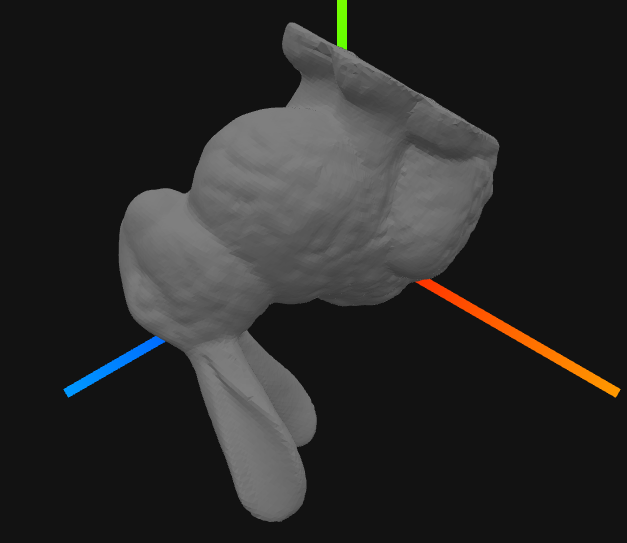
\includegraphics[scale=0.8]{./rendus/original.png}}
\caption{Modèle d'origine}
\end{figure}

\begin{figure}[h!]
\centerline{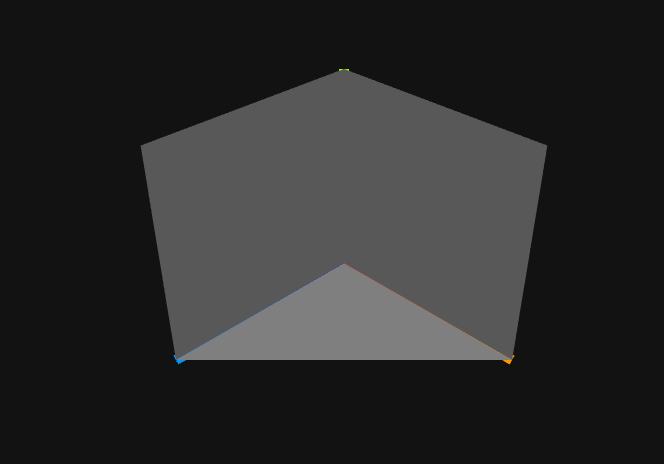
\includegraphics[scale=0.8]{./rendus/pq1.png}}
\caption{PQ = 1}
\end{figure}

\begin{figure}[h!]
\centerline{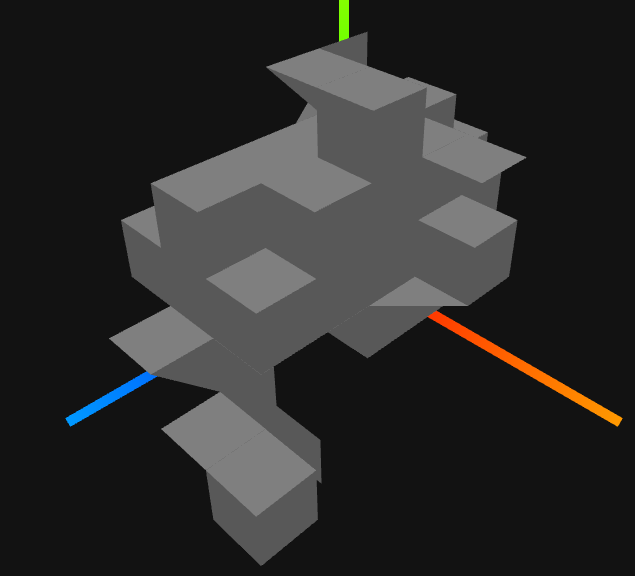
\includegraphics[scale=0.8]{./rendus/pq3.png}}
\caption{PQ = 3}
\end{figure}

\begin{figure}[h!]
\centerline{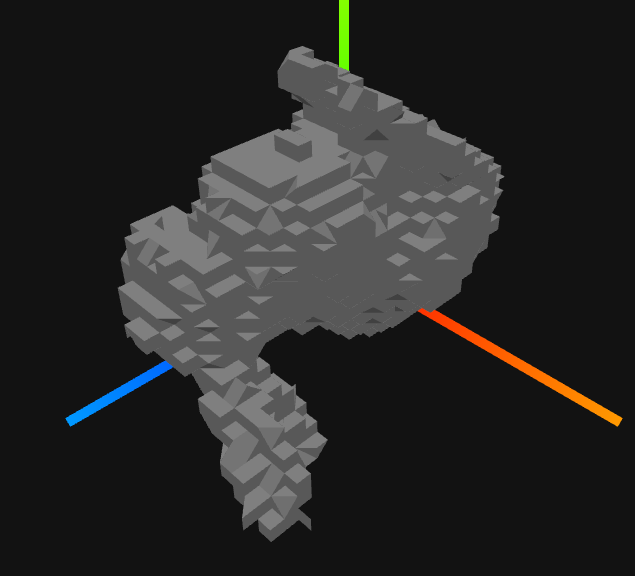
\includegraphics[scale=0.8]{./rendus/pq5.png}}
\caption{PQ = 5}
\end{figure}

\begin{figure}[h!]
\centerline{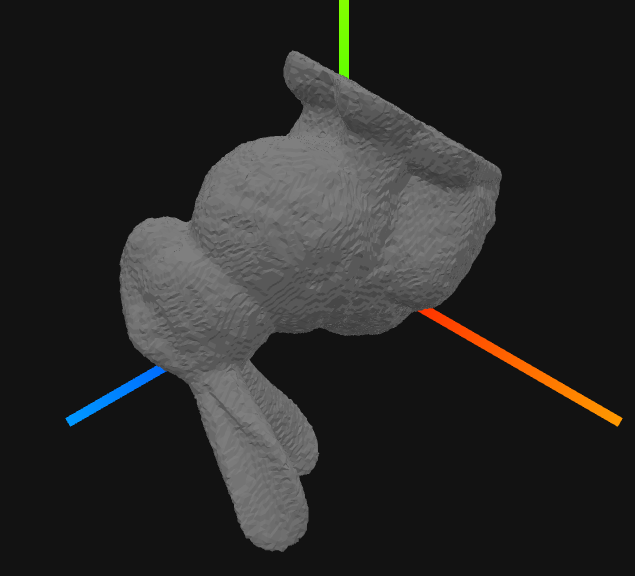
\includegraphics[scale=0.8]{./rendus/pq8.png}}
\caption{PQ = 8}
\end{figure}

\begin{figure}[h!]
\centerline{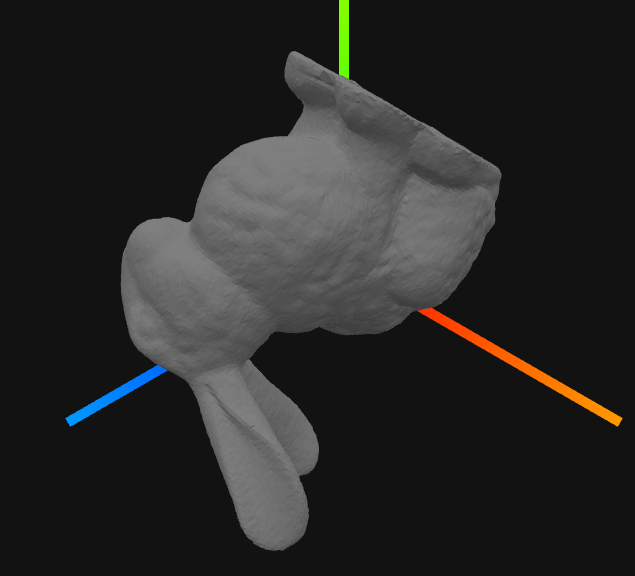
\includegraphics[scale=0.8]{./rendus/pq10.png}}
\caption{PQ = 10}
\end{figure}

\begin{figure}[h!]
\centerline{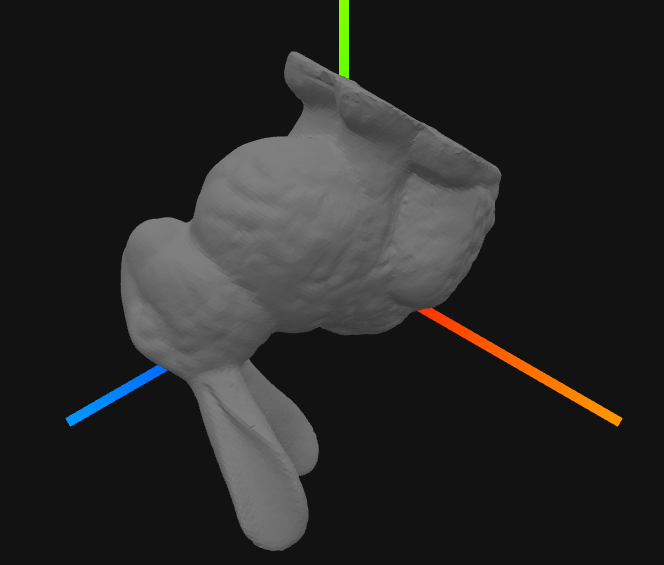
\includegraphics[scale=0.8]{./rendus/pq20.png}}
\caption{PQ = 20}
\end{figure}

\begin{figure}[h!]
\centerline{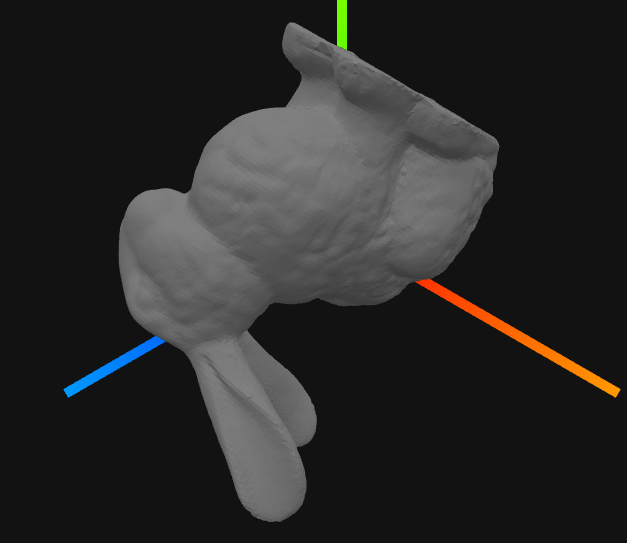
\includegraphics[scale=0.8]{./rendus/pq30.png}}
\caption{PQ = 30}
\end{figure}


\begin{figure}[h!]
\section{RMSE}
Pour calculer le RMSE, on fait la différence entre la coordonée originale et celle quantifiée et déquantifiée on élève cette différence au carré.
On fait ça pour chaque x,y,z de chaque point on fait la somme de tout ces résultats qu'on divise par le nombre de vertex *3. 
Et enfin on on fait la racine carré et on obtient notre RMSE.
\centerline{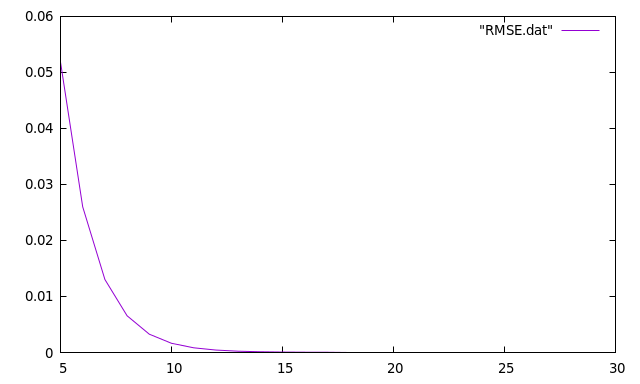
\includegraphics[scale=0.8]{./rendus/rmse.png}}
\caption{Courbe RMSE}
On remarque que la dégradation est imperceptible insignifiante à partir de 15
\end{figure}
 


\end{document}